% Start Paper

\documentclass[11pt,a4paper]{article}
\usepackage[utf8]{inputenc}
\usepackage[pdftex]{graphicx}
\usepackage{CJKutf8, makeidx, listings}

\AtBeginDvi{\input{zhwinfonts}}

\begin{document}
\begin{CJK*}{UTF8}{gbsn}

% 命令
\renewcommand{\abstractname}{摘要}
\newcommand{\HRule}{\rule{\linewidth}{0.5mm}}
\linespread{2.0}

% Title Page

\begin{titlepage}
\begin{center}

% Upper part of the page. The '~' is needed because \\
% only works if a paragraph has started.

\includegraphics[width=0.5\textwidth]{./images/university-logo}\\[1cm]
\textbf{\Huge 贵州大学}\\[1cm]
\textsc{\Large 计算机科学与信息技术学院}\\[1.5cm]

% Title
\HRule\\[0.4cm]
\textbf{\Huge 基于Web的数字报系统设计}\\[0.4cm]
\HRule\\[1.5cm]

% Author and supervisor
\begin{tabular}{ l c r }
  姓名 & 王晓娟 \\[0.2cm]
  学号 & 0908060041 \\[0.2cm]
  班级 & 计科092 \\[0.2cm]
  指导老师 & 吴云 \\[0.2cm]
\end{tabular}

\vfill

{\Large \today}

\end{center}
\end{titlepage}

% 摘要
\begin{abstract}
	% abstract.tex

\noindent
计算机技术的不断发展,互联网技术不断崛起,Web逐渐成为了人们日常生活中不可获取的生命要素。报刊杂志等纸媒作为上一个时代的有利传播工具,将其Web化的步伐已刻不容缓。利用Web快速、精准以及多元化等特性,可以实现一个分众(Focus)、精准(Precise)、互动(Interactive)的多元化平台媒体。

\begin{description}
 	\item[分众] 即用户差异化,服务方有效地区分受众人群
	\item[精准] 即准确把握目标受众的商业需求
	\item[互动] 即能够实现产业链上下游(上游:厂商客户;下游:终端用户)之间的信息互动、相互沟通、互通了解需求,形成有价值的互动信息回馈链条
\end{description}

\indent
而目前亟待解决的问题来自于在思想以及形式上如何从传统媒体平台转换到新媒体平台,现在的解决方案大多分为两类,一类是以电子媒体为主,多以Blog为主,主要战斗力集中在新媒体中与竞争对手进行周旋,在有余力之下,定期地推出某个系列的纸质/电子出版物,其中以SmashingMagzine/iFanr为代表。而另一类则以各大地方报纸、传统媒体行业为主,与前者相反,这些出版社的注意力仍然集中在纸媒体,而在新媒体平台缺乏创新力、创造力的做法,很少能够换得其用户的满堂喝彩。

\indent
本文将会以上述这一问题为根本需求依据,结合在实践中的真实经验,介绍了如何通过Express框架等一系列以ECMAScript为核心的技术体系,进行快速搭建高效、稳定、可迭代的Web应用以及其开发模型。

\noindent
论文共分为七个章节:

\begin{description}
	\item[第一章] 对摘要中的问题进行细致的分析,从企业的角度出发,解决其根本问题
	\item[第二章] 介绍开发平台,包含程序、测试工具、部署平台所使用到的一系列开源工具
	\item[第三章] 从前端出发,说明其架构思路,并提供前端架构图
	\item[第四章] 从后端出发,说明其架构思路,并提供后端架构图
	\item[第五章] 系统的各个组件的设计/实现思路
	\item[第六章] 单独就API设计、缓存以及部署等重要环节,与具体业务场景结合起来一一说明
	\item[第七章] 性能测试与分析
	\item[第八章] 总结该系统的总体设计思路以及发展路线
 	\item[关键字] 数字报刊;NodeJS;MongoDB;系统设计
\end{description}
\end{abstract}

% 第一章 背景
\section{背景与意义}
% ===========================================背景

\subsection{背景}
如前所述,在传统媒介向新媒体转换、融合的阶段中,现存两种实现方式,其一是以数字媒体为主的网络博客,而另一类则是以传统纸媒为主的数字报格式,本系统旨在为后者解决其Web化的工业化难题。

\paragraph{问题描述}

目前大多数数字报的Web化形式都仅停留在了形上,并未真正地融入了Internet元素。

那么什么是Internet,什么又是Web呢,简单地说,就是链接,两者都是增加了链接的数量与质量。例如谷歌、百度,是增进了网民获取所需的链接,而社交网络则是增进了人与人之间的链接,无论是何种形态的Web应用都是以人为出发点,去增进两种事物之间链接的应用程序。

而如今的数字报,从链接上仅仅是增加了一个从头版到文章的链接,但缺少了一个重要的因素,这样的链接并未从人、从用户的角度去考虑,无论是从浏览体验,还是其网络属性来说,都仅仅是将报纸铺在电子显示屏而已。

\noindent
那么真正的Web化是怎样的呢?可以分别从三个方面来逐一体现:
\begin{description}
	\item[分众] 细分用户群,对不同的用户群实现不同的运营策略,要做到这点,需要对用户数据进行收集、建模,为后两方面的实现提供基础数据模型。
	\item[精准] 精准是建立在分众之上,没有很好地细分用户,就没办法精准地了解到特定用户模型的刚性需求。
	\item[互动] 你的用户在使用产品时,需要一个快速、实时的平台与你进行交流,共同改进产品,而这种交流可以是显式的自然语言,同样也可以是其他形式来实现。
\end{description}

\noindent
本章节将会围绕这三个需求,慢慢向你揭开Web化报刊的神秘面纱。

\indent
但对于传统报社,因接不暇地业务需求遽增,同时又要分心涉足互联网,无疑是在蚕食其有限的战斗能力,此时该系统就应运而生,论文最后所实现的这一Web应用即是一个针对广大传统报社的SaaS(Software as a Service)云服务。

\indent
利用这一服务,注册的报社可以轻松地利用已有的资源,生成电子期刊,并获取在线订阅用户,作为一个纯粹的内容提供商(CP, Content Provider)的同时,我们还为报社提供其电子产品的用户数据,方便其针对数字用户制定相应的商业策略。

% ==========需求及系统功能分析===============================================

\subsection{需求及系统功能分析}
\subsubsection{目标用户}
该服务即一综合服务性平台,既拥有上节中说的企业级用户,同时作为一个报刊阅读平台,也拥有着以阅读为目标的个人用户。前者消费流量,而后者提供流量,从而构成了一个良性的生态循环。

\subsubsection{需求分析}
\paragraph{企业级用户}
这类用户的需求相对比较复杂,他们需要的是一个集数字报刊发布软件、数据统计平台为一体的云服务,我们除了提供此类服务之外,还应该尽量地简化他们发布数字报刊的时间成本,提供阅读质量。

\paragraph{个人用户}
这是一类需求相对简单的用户群,它们使用我们服务的理由就是以快速获取信息为主。因此我们需要提供一个各终端平台都无障碍的阅读平台,同时尽力地提高其阅读体验。

\subsubsection{功能分析}
\paragraph{数字报刊发布}
从企业级用户的根本需求出发,以节省其时间代价为根本,极力地简化其发布流程,用户在成功创建一类报刊后,在发布期刊时,仅仅需要上传一份PDF格式文件,我们的服务中心会提用户分析数据,提供适配所有终端的阅读页面。

\paragraph{数字报阅读平台}
从个人用户的根本需求出发,为他们提供一个易于阅读,易于分享的阅读平台。

\paragraph{数据统计平台}
同样为企业级用户量身定做,基于数据可视化技术为企业级用户快速、便捷地筛选出自己想要的信息。

% ==========可行性分析=========================================================

\subsection{可行性分析}
\indent
Occupation

% 第二章 开发平台介绍
\section{开发平台介绍}
% Chapter1 开发平台

\subsection{B/S体系结构}
\indent
B/S体系结构与C/S体系结构相比,不仅具有其大部分优点,还有其不具备的优势
\begin{description}
  \item[开放的标准] B/S所采用的标准都是开放的、非专用的,是经过标准化组织所确定而非单一厂商所制定,保证了应用的通用性与跨平台性。
  \item[开发/维护成本低] B/S应用只需在客户端安装通用的浏览器,维护和升级的工作都在服务端完成,不需要对客户端进行任何改变。
\end{description}
\indent
由以上分析比较可看出,B/S模式具有更遥远的应用前景,它简化开发与维护流程,并适合在网络中发布信息、传播信息。

\begin{figure}[h]
  \centering
    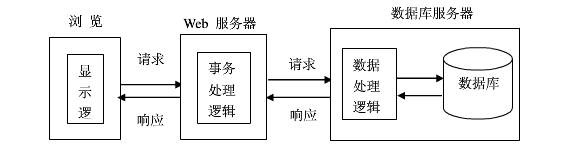
\includegraphics[width=1\textwidth]{./images/bs-graph.png}
  \caption{B/S三层结构图}
\end{figure}

\subsection{开发语言}
\indent
本系统采用了一些相对比较新潮的开发语言,如SeaJS、NodeJS以及MongoDB。其中NodeJS作为HTTP服务器平台,其优点是异步编程模型,使用了异步非阻塞(noblocking I/O)来处理复杂的并发Web请求。为了快速搭建web服务平台上的相关功能,我们选择使用了NodeJS平台上最流行的web开发框架Express,之所以选择它的原因是由于其灵巧的微内核设计方式与插件机制,可以很好地对框架本身的功能进行拓展。

\indent
数据库我们使用了新兴的mongoDB作为数据库服务器平台,它被誉为最接近SQL的NoSQL数据库,既不完全舍弃SQL的一些优秀设计理念,又能够使用NoSQL所带来的高效优势,并且在选择NodeJS客户端驱动时,我们选择了带有模式(Schema)设计的mongoose为主要客户端驱动,也是为了利用SQL的基本设计理论帮助我们保证数据与数据库的可维护性。

\indent
随着前端开发逐步走向工业化的道路,前端模块化会是影响web应用一个重要的因素,而我们使用SeaJS作为前端工业化平台,SeaJS所遵循的CMD规范与NodeJS的模块(Module)兼容性良好,关于前端模块化的详细内容将在后续章节详细说明。

\subsubsection{系统开发环境及工具}
\begin{tabular}{ l c }
  硬盘空间 & 8G及以上 \\
  CPU & 1.7 GHz Intel Core i7 \\
  内存 & 4G \\
  操作系统 & MacOS X \\
  开发平台 & NodeJS/Express \\
  数据库 & MongoDB \\
\end{tabular}

\subsection{NodeJS}

\subsubsection{NodeJS的前世今生}
\indent
NodeJS是一个可以快速构建网络服务及应用的平台。该平台的构建是基于Chrome's JavaScript runtime,也就是说,实际上它是对GoogleV8引擎进行了封装。

V8引 擎执行Javascript的速度非常快,性能非常好。Node对一些特殊用例进行了优化,提供了替代的API,使得V8在非浏览器环境下运行得更好。

V8引擎本身使用了一些最新的编译技术。这使得用Javascript这类脚本语言编写出来的代码与用C这类高级语言写出来的代码性能相差无几,却节省了开发成本。对性能的苛求是Node的一个关键因素。 Javascript是一个事件驱动语言,Node利用了这个优点,编写出可扩展性高的服务器。Node采用了一个称为“事件循环(event loop)”的架构,使得编写可扩展性高的服务器变得既容易又安全。提高服务器性能的技巧有多种多样。Node选择了一种既能提高性能,又能减低开发复杂度的架构。这是一个非常重要的特性。并发编程通常很复杂且布满地雷。Node绕过了这些,但仍提供很好的性能。

Node采用一系列“非阻塞”库来支持事件循环的方式。本质上就是为文件系统、数据库之类的资源提供接口。向文件系统发送一个请求时,无需等待硬盘(寻址并检索文件),硬盘准备好的时候非阻塞接口会通知Node。该模型以可扩展的方式简化了对慢资源的访问, 直观,易懂。尤其是对于熟悉onmouseover、onclick等DOM事件的用户,更有一种似曾相识的感觉。

虽然让Javascript运行于服务器端不是Node的独特之处,但却是其一强大功能。不得不承认,浏览器环境限制了我们选择编程语言的自由。任何服务器与日益复杂的浏览器客户端应用程序间共享代码的愿望只能通过Javascript来实现。虽然还存在其他一些支持Javascript在服务器端 运行的平台,但因为上述特性,Node发展迅猛,成为事实上的平台。

在Node启动的很短时间内,社区就已经贡献了大量的扩展库(模块)。其中很多是连接数据库或是其他软件的驱动,但还有很多是凭他们的实力制作出来的非常有用的软件。

不得不提到的是Node社区。虽然Node项目还非常年轻,但很少看到对一个项目如此狂热的社区。不管是新手,还是专家,大家都围绕着项目,使用并贡献自己的能力,致力于打造一个探索、支持、分享、听取建议的乐土。

\subsubsection{NodeJS的单线程}
\indent
NodeJS中的JavaScript在单线程上执行,但是作为宿主的NodeJS,它本身并非是单线程的,NodeJS在I/O方面动用到一小部分额外的线程协助实现异步。程序员没有机会直接创建线程,因此有人想当然的认为NodeJS的单线程无法很好的利用多核CPU。

\indent
NodeJS封装了内部的异步实现后,导致程序员无法直接操作线程,也就造成所有的业务逻辑运算都会丢到JavaScript的执行线程上,这也就意味着,在高并发请求的时候,I/O的问题是很好的解决了,但是所有的业务逻辑运算积少成多地都运行在JavaScript线程上,形成了一条拥挤的JavaScript运算线程。NodeJS的弱点在这个时候会暴露出来,单线程执行运算形成的瓶颈,拖慢了I/O的效率。这大概可以算得上是密集运算情况下无法很好利用多核CPU的缺点。这条拥挤的JavaScript线程,给I/O形成了性能上限。

\indent
事情又并非绝对的,NodeJS提供了child\_process.fork来创建Node的子进程。在一个Node进程就能很好的解决密集I/O的情况下,fork出来的其余Node子进程可以当作常驻服务来解决运算阻塞的问题(将运算分发到多个Node子进程中上去,与Apache创建多个子进程类似)。当然child\_process机制永远只能解决单台机器的问题,大的Web应用是不可能一台服务器就能完成所有的请求服务的。拜NodeJS在I/O上的优势,跨OS的多Node之间通信的是不算什么问题的。解决NodeJS的运算密集问题的答案其实也是非常简单的,就是将运算分发到多个CPU上。

\subsubsection{基于事件的编程}
\indent
延续上一节的讨论。我们知道NodeJS具有异步的特性,从NodeJS的API设计中可以看出来,任何涉及I/O的操作,几乎都被设计成事件回调的形式,且大多数的类都继承自EventEmitter。这么做的好处有两个,一个是充分利用无阻塞I/O的特性,提高性能;另一个好处则是封装了底层的线程细节,通过事件消息留出业务的关注点给编程者,从而不用关注多线程编程里牵扯到的诸多技术细节。

\indent
事件式编程更贴近于现实生活,是更自然的,所以这种编程风格也导致你的代码跟你的生活一样,是一件复杂的事情。幸运的是,自己的生活要自己去面对,对于一个项目而言,并不需要每个人都去设计整个大业务逻辑,对于架构师而言,业务逻辑是明了的,借助事件式编程带来的业务逻辑松耦合的好处,在设定大框架后,将业务逻辑划分为适当的粒度,对每一个实现业务点的程序员而言,并没有这个痛苦存在。二八原则在这个地方非常有效。

\subsection{Express.js——NodeJS平台上的Web框架}
\indent
Express.js是基于NodeJS,高性能、一流的web开发框架,它通过对NodeJS的部分接口进行重新封装,使其更易于适用在web的世界中,并且提供了良好的插件机制,可以灵活地向应用中添加模版引擎,中间件等,因而使其具有一定的生态活力。

\subsection{NoSQL与MongoDB}
\indent
随着互联网web2.0网站的兴起,非关系型的数据库成了一个极其热门的新领域,非关系数据库产品的发展非常迅速。而传统的关系数据库在应付web2.0网站,特别是超大规模和高并发的SNS类型的web2.0纯动态网站已经显得力不从心,暴露了很多难以克服的问题,例如:

\begin{description}
    \item[对数据库高并发读写的需求] web2.0网站要根据用户个性化信息来实时生成动态页面和提供动态信息,所以基本上无法使用动态页面静态化技术,因此数据库并发负载非常高,往往要达到每秒上万次读写请求。关系数据库应付上万次SQL查询还勉强顶得住,但是应付上万次SQL写数据请求,硬盘IO就已经无法承受了。其实对于普通的BBS网站,往往也存在对高并发写请求的需求。
    \item[对海量数据的高效率存储和访问的需求] 对于大型的SNS网站,每天用户产生海量的用户动态,以国外的Friendfeed为例,一个月就达到了2.5亿条用户动态,对于关系数据库来说,在一张2.5亿条记录的表里面进行SQL查询,效率是极其低下乃至不可忍受的。再例如大型web网站的用户登录系统,例如腾讯,盛大,动辄数以亿计的帐号,关系数据库也很难应付。
    \item[对数据库的高可扩展性和高可用性的需求] 在基于web的架构当中,数据库是最难进行横向扩展的,当一个应用系统的用户量和访问量与日俱增的时候,你的数据库却没有办法像web server和app server那样简单的通过添加更多的硬件和服务节点来扩展性能和负载能力。对于很多需要提供24小时不间断服务的网站来说,对数据库系统进行升级和扩展是非常痛苦的事情,往往需要停机维护和数据迁移,为什么数据库不能通过不断的添加服务器节点来实现扩展呢?
\end{description}

\noindent
在上面提到的“三高”需求面前,关系数据库遇到了难以克服的障碍,而对于web2.0网站来说,关系数据库的很多主要特性却往往无用武之地,例如:

\begin{description}
    \item[数据库事务一致性需求] 很多web实时系统并不要求严格的数据库事务,对读一致性的要求很低,有些场合对写一致性要求也不高。因此数据库事务管理成了数据库高负载下一个沉重的负担。
    \item[数据库的写实时性和读实时性需求] 对关系数据库来说,插入一条数据之后立刻查询,是肯定可以读出来这条数据的,但是对于很多web应用来说,并不要求这么高的实时性。
    \item[对复杂的SQL查询,特别是多表关联查询的需求] 任何大数据量的web系统,都非常忌讳多个大表的关联查询,以及复杂的数据分析类型的复杂SQL报表查询,特别是SNS类型的网站,从需求以及产品设计角度,就避免了这种情况的产生。往往更多的只是单表的主键查询,以及单表的简单条件分页查询,SQL的功能被极大的弱化了。
\end{description}

\noindent
因此,关系数据库在这些越来越多的应用场景下显得不那么合适了,为了解决这类问题的非关系数据库应运而生。

NoSQL 是非关系型数据存储的广义定义。它打破了长久以来关系型数据库与ACID理论大一统的局面。NoSQL 数据存储不需要固定的表结构,通常也不存在连接操作。在大数据存取上具备关系型数据库无法比拟的性能优势。该术语在 2009 年初得到了广泛认同。

\paragraph{MongoDB}
是一个介于关系数据库和非关系数据库之间的产品,是非关系数据库当中功能最丰富,最像关系数据库的。他支持的数据结构非常松散,是类似json的bson格式,因此可以存储比较复杂的数据类型。Mongo最大的特点是他支持的查询语言非常强大,其语法有点类似于面向对象的查询语言,几乎可以实现类似关系数据库单表查询的绝大部分功能,而且还支持对数据建立索引。它的特点是高性能、易部署、易使用,存储数据非常方便。

\noindent
主要功能特性有:
\begin{itemize}
  \item 面向集合存储,易存储对象类型的数据。
  \item 模式自由。
  \item 支持动态查询。
  \item 支持完全索引,包含内部对象。
  \item 支持查询。
  \item 支持复制和故障恢复。
  \item 使用高效的二进制数据存储,包括大型对象(如视频等)。
  \item 自动处理碎片,以支持云计算层次的扩展性。
  \item 支持RUBY,PYTHON,JAVA及NodeJS等多种语言。
  \item 文件存储格式为BSON(一种JSON的扩展)。
  \item 可通过网络访问。
\end{itemize}

\indent
所谓“面向集合”(Collection-Oriented),意思是数据被分组存储在数据集中,被称为一个集合(Collection)。每个集合在数据库中都有一个唯一的标识名,并且可以包含无限数目的文档。集合的概念类似关系型数据库(RDBMS)里的表(table),不同的是它不需要定义任何模式(schema)。

\indent
模式自由(schema-free),意味着对于存储在mongodb数据库中的文件,我们不需要知道它的任何结构定义。如果需要的话,你完全可以把不同结构的文件存储在同一个数据库里。

\indent
存储在集合中的文档,被存储为键-值对的形式。键用于唯一标识一个文档,为字符串类型,而值则可以是各种复杂的文件类型。我们称这种存储形式为BSON(Binary Serialized dOcument Format)。

\subsection{SeaJS前端平台}
\indent
SeaJS是一个遵循CommonJS规范的JavaScript模块加载框架,可以实现其的模块化开发及加载机制。与jQuery等框架不同,SeaJS不会扩展封装语言特性,而只是实现JavaScript的模块化及按模块加载。SeaJS的主要目的是令JavaScript开发模块化并可以轻松愉悦进行加载,将前端工程师从繁重的JavaScript文件及对象依赖处理中解放出来,可以专注于代码本身的逻辑。SeaJS可以与jQuery这类框架完美集成。使用SeaJS可以提高JavaScript代码的可读性和清晰度,解决目前JavaScript编程中普遍存在的依赖关系混乱和代码纠缠等问题,方便代码的编写和维护。\\[0.1cm]
\indent
SeaJS的作者是淘宝前端工程师玉伯。\\
\indent
SeaJS本身遵循KISS(Keep It Simple, Stupid)理念进行开发,其本身仅有个位数的API,因此学习起来毫无压力。在学习SeaJS的过程中,处处能感受到KISS原则的精髓——仅做一件事,做好一件事。

\textbf{RequireJS与SeaJS}
\par
RequireJS作为Javascript模块化开发中的前辈,与SeaJS都是模块加载器,倡导模块化开发理念,核心价值是让JavaScript的模块化开发变得简单自然。而二者的区别是:
\begin{description}
  \item[定位有差异] RequireJS 想成为浏览器端的模块加载器,同时也想成为 Rhino / Node 等环境的模块加载器。Sea.js 则专注于 Web 浏览器端,同时通过 Node 扩展的方式可以很方便跑在 Node 环境中
  \item[遵循的规范不同] RequireJS 遵循 AMD(异步模块定义)规范,Sea.js 遵循 CMD (通用模块定义)规范。规范的不同,导致了两者 API 不同。Sea.js 更贴近 CommonJS Modules/1.1 和 Node Modules 规范。
  \item[推广理念有差异] RequireJS 在尝试让第三方类库修改自身来支持 RequireJS,目前只有少数社区采纳。Sea.js 不强推,采用自主封装的方式来“海纳百川”,目前已有较成熟的封装策略
  \item[对开发调试的支持有差异] Sea.js 非常关注代码的开发调试,有 nocache、debug 等用于调试的插件。RequireJS 无这方面的明显支持
  \item[插件机制不同] RequireJS 采取的是在源码中预留接口的形式,插件类型比较单一。Sea.js 采取的是通用事件机制,插件类型更丰富。
\end{description}

\clearpage

% 第三章 服务端架构细节
\section{服务端架构细节}
% Chapter 服务端架构细节

\subsection{NodeJS+MongoDB架构优势}
\indent
Occupation

\subsection{模块对象设计}
\indent
由于使用的是基于ECMAScript262的NodeJS为基本开发语言,因此并没有传统面向对象中的类,但并不能说其不支持面向对象的特性。我基于Express.js开发了一个数据库连接工具——express-model,另外它也是一个建模工具,系统中所有的模型都被放在根目录下一个叫models的文件夹中,下面分别对其中的文件进行描述。

\subsubsection{express-model}
在描述对象模型之前,先来看看如何使用express-model,首先是更加仔细地对它进行一段描述:它为Express框架提供Model支持,可集成多种数据库(SQL \& NoSQL),灵活性高的轻量级工具。 由于Express官方并未显式地提供Model支持,express-model不仅能有效嵌入Express Mvc中,还支持多种需要Model的场景。

\clearpage

\noindent
\texttt{\large 创建一个Model:}

% create a model in express-model

\lstset{language=C}

\begin{lstlisting}[frame=single]
Models.define('yourModelName', function(exports) {
	exports.name = 'express-model 1.0'
	exports.getName = function() {
		return this.name
	}
})
\end{lstlisting}
~

\noindent
\texttt{\large 使用Model:}

% use a model in express-model

\lstset{language=C}

\begin{lstlisting}[frame=single]
var model = Models.use('yourModelName', function() {
	this.someVariable_1 = 1;
	this.someVariable_2 = 2;
})
response.render('yourViewName', model)
\end{lstlisting}

\subsubsection{user.js}

\noindent
\texttt{\large 其模型定义代码如下:}

% use a model in express-model

\lstset{language=C}

\begin{lstlisting}[frame=single]
var UserSchema = new Db.Schema({
	name: String,
	email: String,
	password: String,
	role: String
})
UserSchema.index({ name: 1, role: 1 })
\end{lstlisting}

\subsubsection{groups.js}

\noindent
\texttt{\large 其模型定义代码如下:}

% use a model in express-model

\lstset{language=C}

\begin{lstlisting}[frame=single]
var GroupSchema = new Db.Schema({
	content: [ String ]
}, {
	collection: 'groups'
})
\end{lstlisting}

\subsubsection{kan.js}

\noindent
\texttt{\large 其模型定义代码如下:}

% use a model in express-model

\lstset{language=C}

\begin{lstlisting}[frame=single]
var KanSchema = new Db.Schema({
	user: String,
	name: String,
	group: String,
	tags: String,
	description: String,
	cover: String
})
KanSchema.index({name: 1, group: 1})
\end{lstlisting}

\subsubsection{issue.js}

\noindent
\texttt{\large 其模型定义代码如下:}

% use a model in express-model

\lstset{language=C}

\begin{lstlisting}[frame=single]
var IssueSchema = new Db.Schema({
	title: String,
	type: Boolean,
	content: String,
	date: Date,
	kanId: String,
})
IssueSchema.index({kan: 1})
\end{lstlisting}

\subsection{数据库设计}
\indent
Occupation

\subsection{服务器(组)选型}
\indent
Occupation

\subsection{服务端架构图}
\indent
Occupation

% 第四章 前端架构细节
\section{前端架构细节}
% Chapter1 前端架构细节

\subsection{模块化的前端开发}
\indent
Occupation

\subsection{拥抱SeaJS}
\indent
Occupation

\subsection{前端UI库——bootstrap.js}
\indent
Occupation

\subsection{前端架构图}
\indent
Occupation


\clearpage

% 第五章 系统功能实现
\section{系统功能实现}
% 系统功能实现

\subsection{用户/组}
\indent
Occupation

\subsection{发布平台}
\indent
Occupation

\subsection{在线阅读}
\indent
Occupation


\clearpage

% 第六章 核心功能实现
\section{核心功能实现}
% Chapter1 核心功能实现

\subsection{API设计}
\indent
Occupation

\subsection{缓存设计}
\indent
Occupation

\subsection{部署设计}
\indent
Occupation

% 第七章 性能测试与分析
\section{性能测试与分析}
% Chapter1 测试

\subsection{测试工具介绍}
\indent
Occupation

\subsection{前端性能}
\indent
Occupation

\subsection{服务器性能}
\indent
Occupation

% 第八章 总结
\section{总结}
% Chapter8 总结

\indent
Occupation

% 致谢
\section{致谢}
\indent
Occupation

\end{CJK*}
\end{document}

% End Paper